\documentclass[12pt]{article}
\setlength{\oddsidemargin}{0in}
\setlength{\evensidemargin}{0in}
\setlength{\textwidth}{6.5in}
\setlength{\parindent}{0in}
\setlength{\parskip}{\baselineskip}

\usepackage{amsmath,amsfonts,amssymb,graphicx, hyperref, float}

\begin{document}

IBEHS 4A03 \hfill Assignment \#3\\
Baoze Lin, Hady Ibrahim

\hrulefill

% Custom numbering for subparts (e.g., 2.1, 2.2)
\renewcommand{\theenumii}{\arabic{enumi}.\arabic{enumii}}

\begin{enumerate}
\item Question 1
  \begin{enumerate}
    % Answer to 1.1
    \item
    The open-loop step response of the system is shown in the Simulink model (Figure \ref{fig:figure1_1}) below with the response shown in Figure \ref{fig:figure1_2}.
    
    \begin{figure}[H]
      \centering
      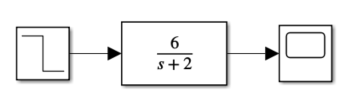
\includegraphics[width=0.3\textwidth]{Figures/Models/model1_1.png}
      \caption{Simulink model of the open-loop step response}
      \label{fig:figure1_1}
    \end{figure}

    \begin{figure}[H]
      \centering
      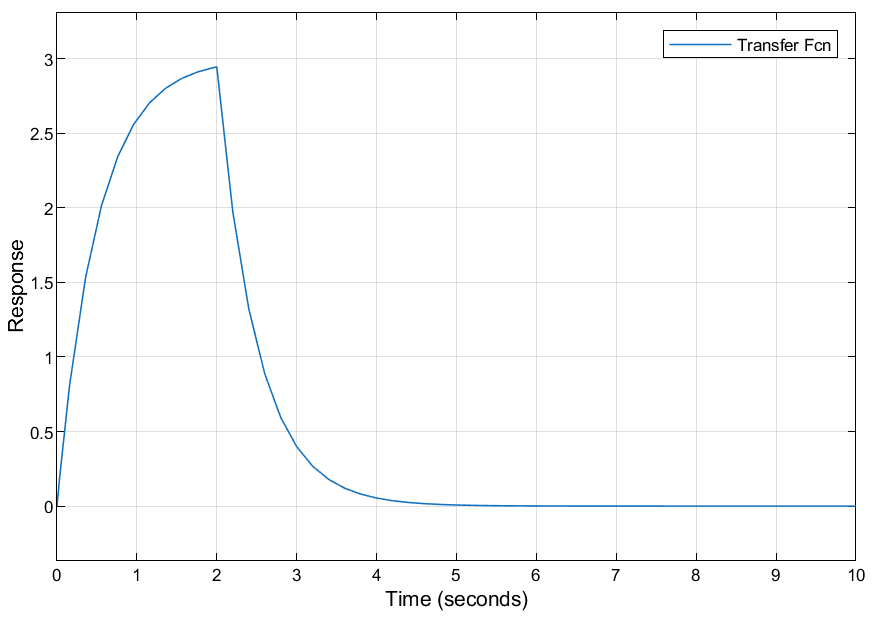
\includegraphics[width=0.5\textwidth]{Figures/figure1_1.png}
      \caption{Open-loop step response}
      \label{fig:figure1_2}
    \end{figure}

    To identify the gain and time constant for this system, we can rearrange the transfer function to isolate the gain K and time constant $\tau$:

    The given transfer function is:
    \[
    G_p(s) = \frac{6}{s + 2}
    \]

    To express this in the standard first-order form, which is:
    \[
    G(s) = \frac{K}{\tau s + 1}
    \]
    where \( K \) is the gain and \( \tau \) is the time constant.

    We rearrange \( G_p(s) \) as follows:
    \[
    G_p(s) = \frac{6}{2(\frac{1}{2}s + 1)} = \frac{3}{\frac{1}{2}s + 1}
    \]

    Thus, we identify the gain \( K \) and the time constant \( \tau \) as:
    \[
    K = 3, \quad \tau = \frac{1}{2}
    \]

    % Answer to 1.2
    \item 
    The closed-loop feedback control with a proportional controller is shown below in Figure \ref{fig:figure1_3}. The transfer function $G_c(s)$ can also be represented by a proportional gain $K_c$.

    \begin{figure}[H]
      \centering
      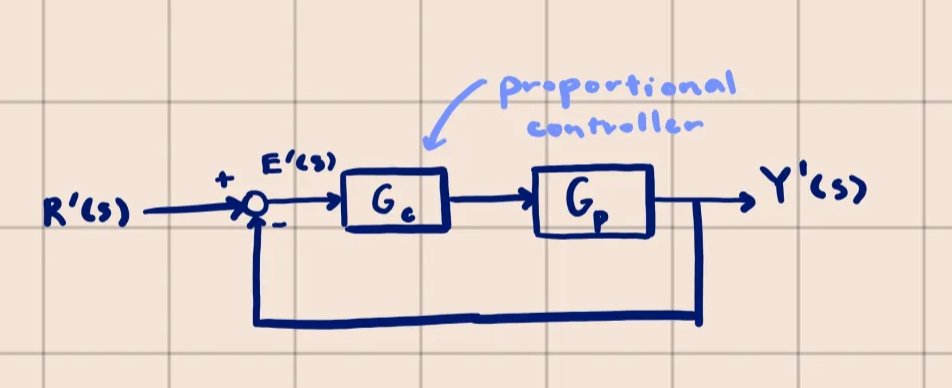
\includegraphics[width=0.7\textwidth]{Figures/Models/model1_2.png}
      \caption{Simulink model of the closed-loop feedback control with a proportional controller}
      \label{fig:figure1_3}
    \end{figure}
    
    \pagebreak
    
    % Answer to 1.3
    \item 
    The Simulink model is shown below in Figure \ref{fig:figure1_4}. The response of the system is shown in Figure \ref{fig:figure1_5}.

    \begin{figure}[H]
      \centering
      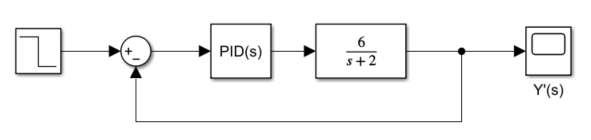
\includegraphics[width=0.5\textwidth]{Figures/Models/model1_3.png}
      \caption{Simulink model of the closed-loop feedback control with a proportional controller}
      \label{fig:figure1_4}
    \end{figure}

    \begin{figure}[H]
      \centering
      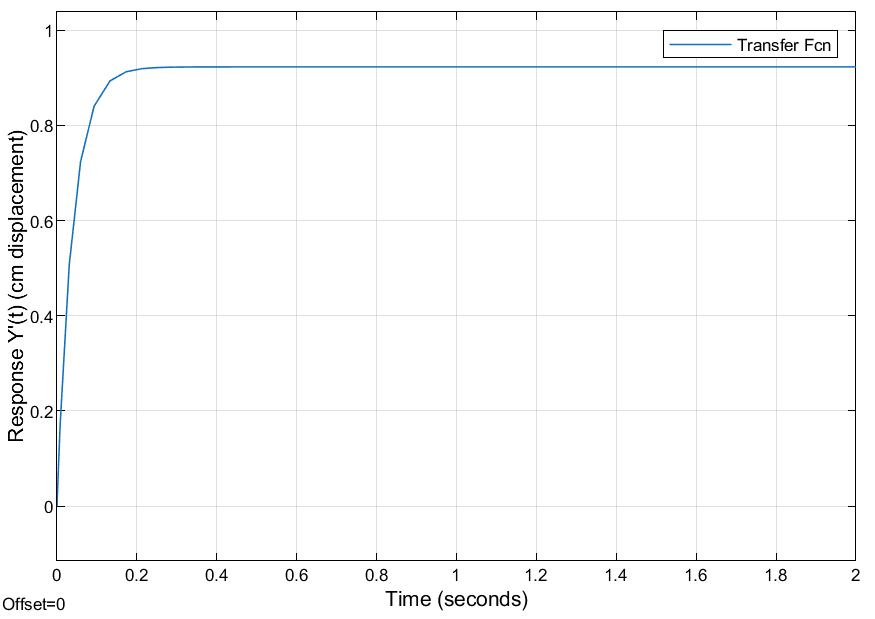
\includegraphics[width=0.8\textwidth]{Figures/figure1_3.png}
      \caption{Closed-loop step response}
      \label{fig:figure1_5}
    \end{figure}

    % Answer to 1.4
    \item
    The closed-loop transfer function \( T(s) \) is given by:
    \[
    T(s) = \frac{Y'(s)}{R'(s)} = \frac{G_c(s)G_p(s)}{1 + G_c(s)G_p(s)}
    \]

    Where \( G_c(s) = K_c = 4 \) (proportional controller) and \( G_p(s) = \frac{6}{s+2} \) (plant transfer function). Substituting the transfer functions:
    \[
    T(s) = \frac{4 \cdot \frac{6}{s+2}}{1 + 4 \cdot \frac{6}{s+2}}
    \]

    Simplifying:
    \[
    T(s) = \frac{\frac{24}{s+2}}{1 + \frac{24}{s+2}} = \frac{24}{s+2+24} = \frac{24}{s+26}
    \]

    Thus, the closed-loop transfer function is:
    \[
    T(s) = \frac{24}{s+26}
    \]

    We then apply the Final Value Theorem, which states that:
    \[
    \lim_{t \to \infty} y(t) = \lim_{s \to 0} sY(s)
    \]

    For a unit step input \( R'(s) = \frac{1}{s} \), the Laplace transform of the output is:
    \[
    Y'(s) = T(s)R'(s) = \frac{24}{s+26} \cdot \frac{1}{s}
    \]

    Applying the FVT:
    \[
    \lim_{t \to \infty} y(t) = \lim_{s \to 0} s \cdot \frac{24}{(s+26)s} = \lim_{s \to 0} \frac{24}{s+26} = \frac{24}{26} = \frac{12}{13} \approx 0.923
    \]

    The steady-state value of the output is approximately \( 0.923 \). Since the system is operating on displacement from a rock assembly with a step input, the set point is 1. Thus, the offset of this system is approximately \( 0.923 \). Referring to the step response in Figure \ref{fig:figure1_5}, we can see the offset is approximately \( 1 - 0.923 = 0.077\).

    \pagebreak

    % Answer to 1.5
    \item
    The closed-loop system for controller gains $K_c = {0.25, 1, 2, 4, 10}$ are shown in Figure \ref{fig:figure1_6}. Observing the results, we can see that the offset of the system decreases as the proportional gain increases.

    \begin{figure}[H]
      \centering
      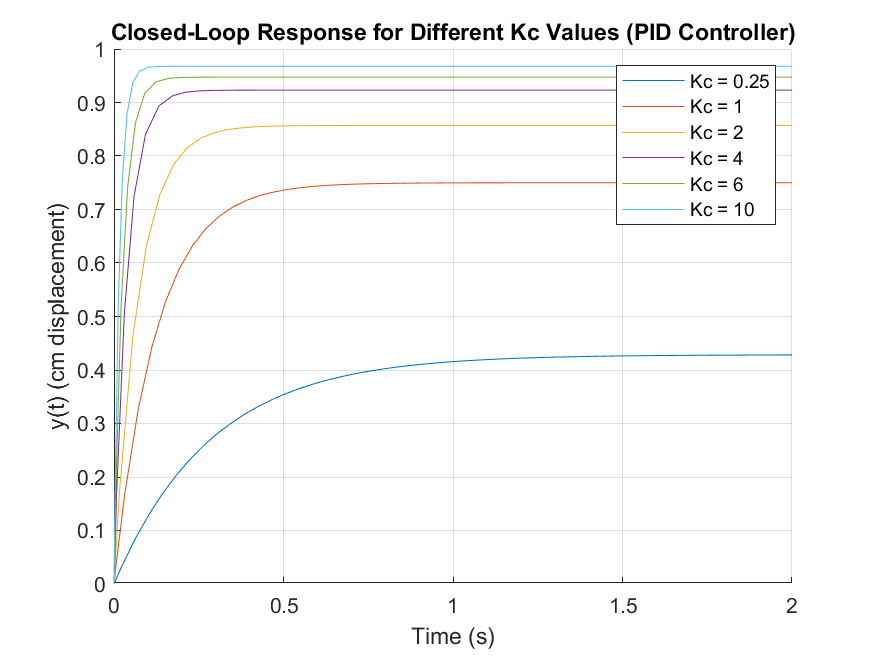
\includegraphics[width=0.8\textwidth]{Figures/figure1_5.png}
      \caption{Closed-loop step response for different controller gains}
      \label{fig:figure1_6}
    \end{figure}

    % Answer to 1.6
    \item
    We want to find the controller gain \(K_c\) such that the offset is less than 0.08. The offset is given by:

    \[
    \text{Offset} = \lim_{t \to \infty} (r(t) - y(t))
    \]

    Using the Final Value Theorem:

    \[
    \text{Offset} = \lim_{s \to 0} \left(1 - \frac{K_c \cdot G_p}{1 + K_c \cdot G_p}\right)
    \]

    With \(G_p = \frac{6}{s+2}\), we evaluate at \(s=0\):

    \[
    \text{Offset} = 1 - \frac{K_c \cdot \frac{6}{0+2}}{1 + K_c \cdot \frac{6}{0+2}} = 1 - \frac{3K_c}{1 + 3K_c}
    \]

    We require that the offset be less than 0.08:

    \[
    0.08 > 1 - \frac{3K_c}{1 + 3K_c}
    \]

    Rearranging the inequality:

    \[
    \frac{3K_c}{1 + 3K_c} > 1 - 0.08 = 0.92
    \]

    \[
    3K_c > 0.92(1 + 3K_c)
    \]

    \[
    K_c > 3.8333...
    \]

    Therefore, the controller gain \(K_c\) must be greater than approximately 3.83 to achieve an offset less than 0.08.

    % Answer to 1.7
    \item
    We change from the proportional controller to the proportional-integral controller by adjusting the transfer function \(G_c(s)\) to include an integral term. The transfer function for the PI controller is given by:

    \[
    G_c(s) = K_c \left(1 + \frac{1}{\tau_I s}\right)
    \]

    Where \(K_c = 3\) and \(\tau_I = 0.05\).  The response of the system is shown in Figure \ref{fig:figure1_7}.

    \begin{figure}[H]
      \centering
      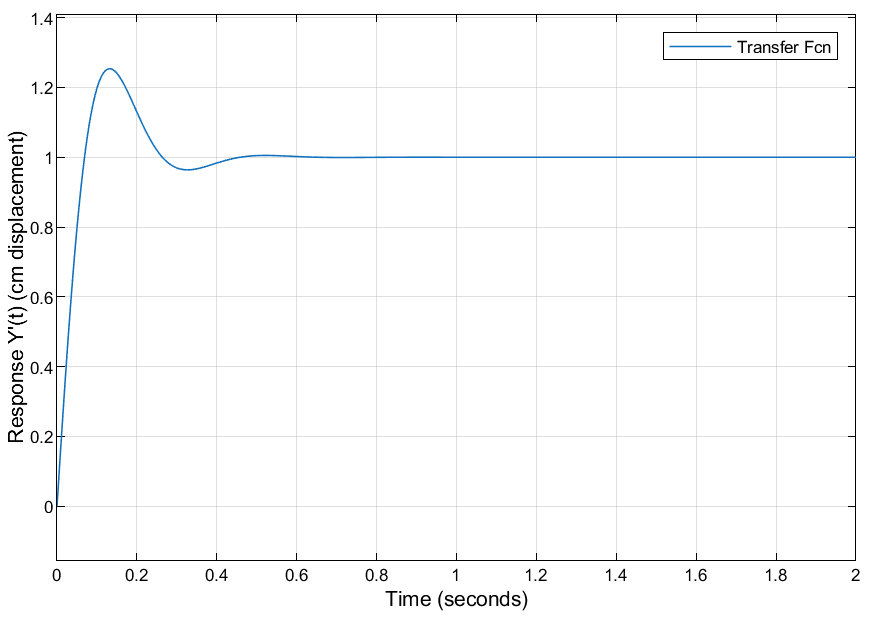
\includegraphics[width=0.8\textwidth]{Figures/figure1_7.png}
      \caption{Closed-loop step response with a PI controller}
      \label{fig:figure1_7}
    \end{figure}

    % Answer to 1.8
    \item
    Given the below two transfer functions in our system:

    \[
    G_c = K_c \left( 1 + \frac{1}{\tau_I s} \right)
    \]

    \[
    G_p = \frac{6}{s+2} = \frac{K_p}{\tau_p s + 1}
    \]

    where,

    \[
    K_p = 3, \quad \tau_p = \frac{1}{2}, \quad K_c = 3, \quad \tau_I = 0.05
    \]

    Together, the closed-loop transfer function for the system becomes:

    \[
    \frac{Y'(s)}{R'(s)} = \frac{\tau_I s + 1}{\frac{\tau_I \tau_p}{K_c K_p} s^2 + \tau_I \frac{(1 + K_c K_p)}{K_c K_p} s + 1}
    \]

    We can use the equations as presented in the lecture to calculate the time constant \( \tau \) and the damping factor \( \zeta \).

    \[
    \tau = \sqrt{\frac{\tau_I \tau_p}{K_c K_p}} = \sqrt{\frac{(0.05)(\frac{1}{2})}{(3)(3)}}
    = \sqrt{0.00278}
    \]

    \[
    \tau \approx 0.0527
    \]

    \[
    \zeta = \frac{1}{2} (1 + K_c K_p) \sqrt{\frac{\tau_I}{K_c K_p \tau_p}}
 = \frac{1}{2} (1 + 9) \sqrt{\frac{0.05}{(3)(3)(\frac{1}{2})}}
    \]

    \[
    \zeta \approx 0.526
    \]

    We also derive the closed-loop gain \( K \).

    \[
    K = \tau_I s + 1 = 0.05s + 1
    \]

    The calculated time constant is approximately \( \tau \approx 0.0527 \), which suggests the system should settle relatively quickly. The expected settling time, approximately \( 4\tau = 0.21s \), can be seen in Figure \ref{fig:figure1_7}, where it settles around that point. \linebreak

    The damping factor was found to be \( \zeta \approx 0.526 \), suggesting a slightly underdamped response. This means the system should exhibit small oscillations but should not overshoot excessively, as observed in the above figure. \linebreak

    The closed-loop gain is given by \( K = 0.05s + 1 \), which means the gain varies with frequency rather than being a simple constant. Evaluating it at steady-state (\( s = 0 \)), we get \( K(0) = 1 \), which confirms that the system should track a step input without steady-state error. Over time, our system approaches 1 as expected.

    % Answer to 1.9
    \item
    The closed-loop system for integral times \( \tau_I = {0.01, 0.05, 0.1, 0.5, 1, 2} \) are shown in Figure \ref{fig:figure1_8}. As the integral time decreases, the system has an increased speed of response but also a higher relative overshoot.

    \begin{figure}[H]
      \centering
      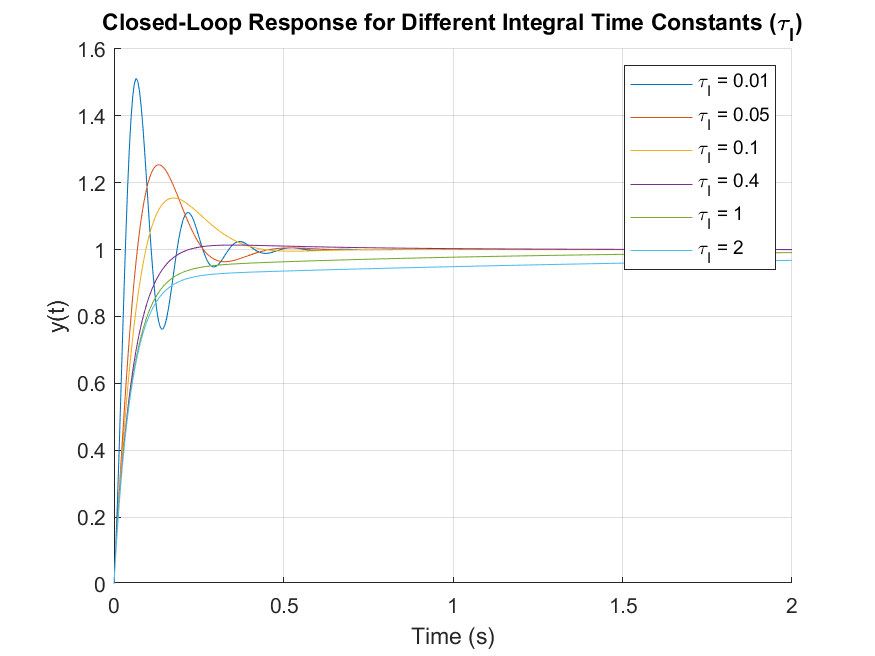
\includegraphics[width=0.8\textwidth]{Figures/figure1_9.png}
      \caption{Closed-loop step response for different integral times}
      \label{fig:figure1_8}
    \end{figure}

    From comparing the different integral time constants, we can see that \(\tau_I\) dictates in a PI controller the trade-off between response speed and stability. Small values (e.g., \(\tau_I = 0.01\)) yield fast responses but can cause excessive overshoot and oscillations. Larger values (e.g., \(\tau_I = 2\)) improve stability with less overshoot but result in slower responses. Tuning \(\tau_I\) aims to find an optimal value, like \(\tau_I = 0.4\), that balances speed and stability according to the specific process requirements. This is due to the mathematical relationship between \(\tau_I\) and the damping factor and time constant, which affect the system's response characteristics.

    % Answer to 1.10
    \item
    The surface plots are shown below in Figure \ref{fig:figure1_9} and Figure \ref{fig:figure1_10}. The surface plots show the relationship between the integral time constant \( \tau_I \) and the damping factor \( \zeta \) with the settling time and the relative overshoot.

    \begin{figure}[H]
      \centering
      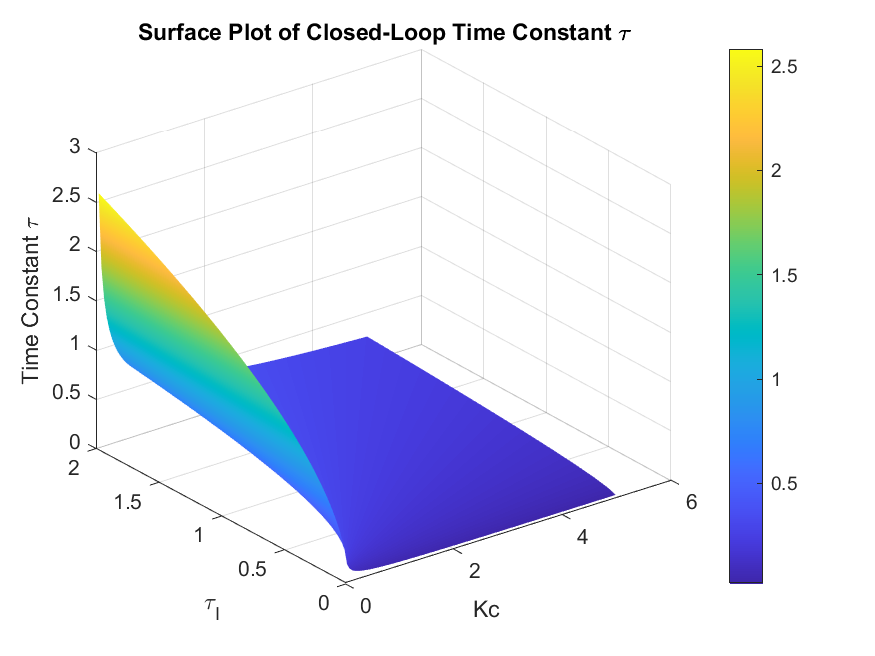
\includegraphics[width=0.6\textwidth]{Figures/figure1_10a.png}
      \caption{Surface plot of settling time and integral time constant}
      \label{fig:figure1_9}
    \end{figure}

    \begin{figure}[H]
      \centering
      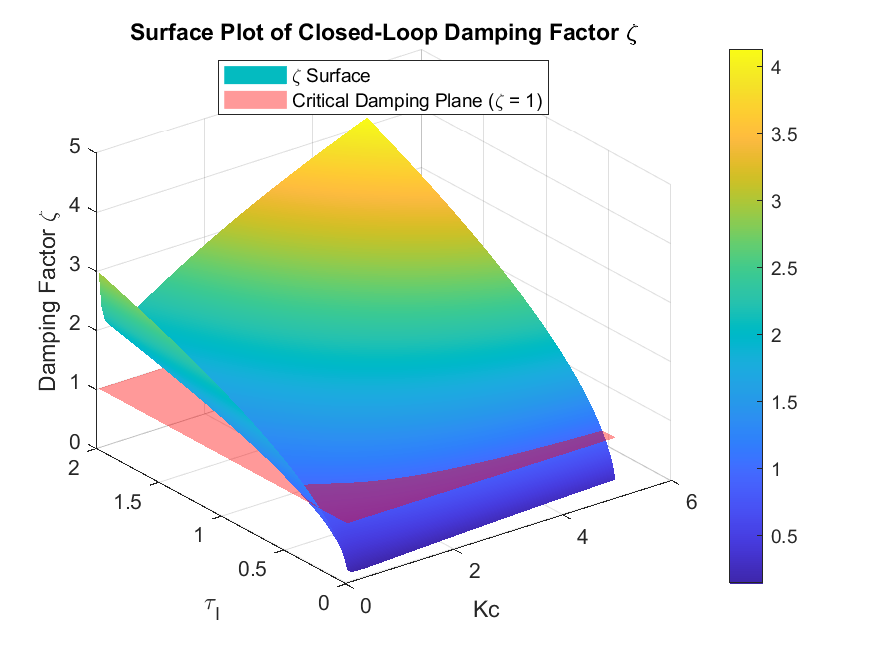
\includegraphics[width=0.6\textwidth]{Figures/figure1_10b.png}
      \caption{Surface plot of relative overshoot and integral time constant}
      \label{fig:figure1_10}
    \end{figure}

    The surface plots for the closed-loop time constant (\(\tau\)) and damping factor (\(\zeta\)) reveal important insights into the system's dynamics and the trade-offs between speed and stability. The time constant plot shows that \(\tau\) decreases as the proportional gain (\(K_c\)) increases, indicating a faster system response. However, very high \(K_c\) values can lead to instability, as seen in the damping factor plot. Similarly, smaller integral time constants (\(\tau_I\)) reduce \(\tau\), but overly small \(\tau_I\) can destabilize the system. The goal is to minimize \(\tau\) for a fast response while ensuring the system remains stable.

    The damping factor plot highlights that a value of \(\zeta\) close to 1 is ideal, as it represents critical damping, where the system responds quickly without oscillations. For small \(K_c\), the system is underdamped (\(\zeta < 1\)), leading to oscillations, while very large \(K_c\) results in overdamping (\(\zeta > 1\)), causing a sluggish response. Larger \(\tau_I\) values increase \(\zeta\), while smaller \(\tau_I\) reduce it, potentially leading to instability.

    To optimize the system, we aim to balance speed and stability by selecting \(K_c\) and \(\tau_I\) values that minimize \(\tau\) while keeping \(\zeta\) close to 1. From the plots, moderate \(K_c\) values (e.g., 2–4) and small-to-moderate \(\tau_I\) values (e.g., 0.5–1) are likely to achieve this balance, providing a fast and stable response.

    % Answer to 1.11
    \item
    The curve that represents the intersection between the surface $\zeta = f(K_c, \tau_I)$ and plane $\zeta = 1$. The curve is shown in Figure \ref{fig:figure1_11}.

    \begin{figure}[H]
      \centering
      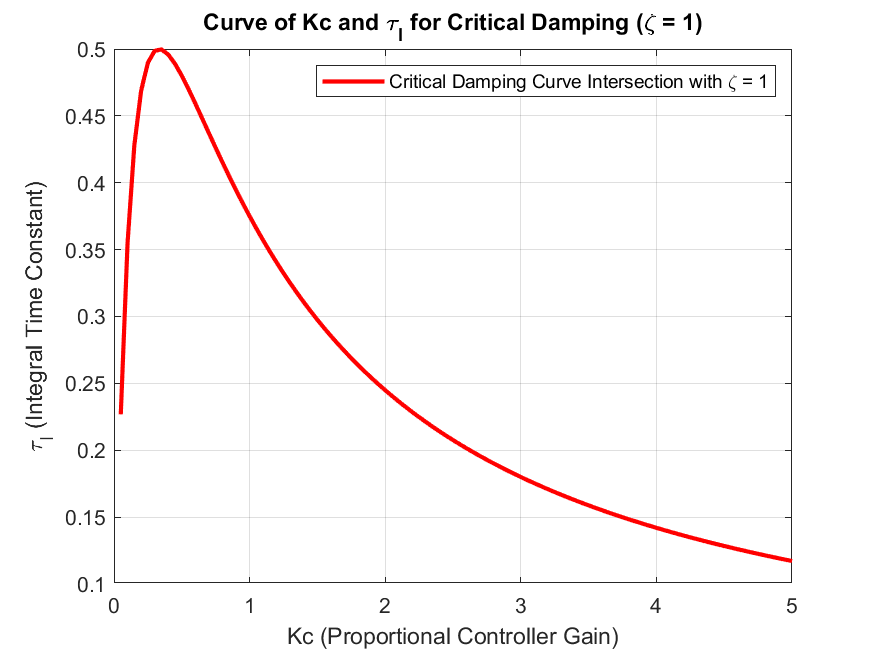
\includegraphics[width=0.7\textwidth]{Figures/figure1_11.png}
      \caption{Intersection curve between the surface and plane}
      \label{fig:figure1_11}
    \end{figure}


  \end{enumerate}

  

\pagebreak

\item Question 2
  \begin{enumerate}
    \item placeholder
  \end{enumerate}

\end{enumerate}

\end{document}
